\documentclass[a4paper,11pt,UTF8]{article}
\usepackage{ctex}
\usepackage{amsmath,amsthm,amssymb,amsfonts}
\usepackage{amsmath}
\usepackage[a4paper]{geometry}
\usepackage{graphicx}
\usepackage{microtype}
\usepackage{siunitx}
\usepackage{booktabs}
\usepackage[colorlinks=false, pdfborder={0 0 0}]{hyperref}
\usepackage{cleveref}
\usepackage{esint} 
\usepackage{graphicx}
\usepackage{ragged2e}
\usepackage{pifont}
\usepackage{extarrows}
\usepackage{mathptmx}
\usepackage{float}
\usepackage{caption}
\usepackage{subfigure}

\captionsetup[figure]{name={Figure}}

\title{Microelectronics Circuit Analysis and Design Homework(14th)}
\author{Yuejin Xie \quad U202210333}
\date{Nov 12nd, 2023}
\begin{document}
\maketitle
Analysis circuit, determine the voltage gain:

1.
\begin{figure}[H]
	\centering
	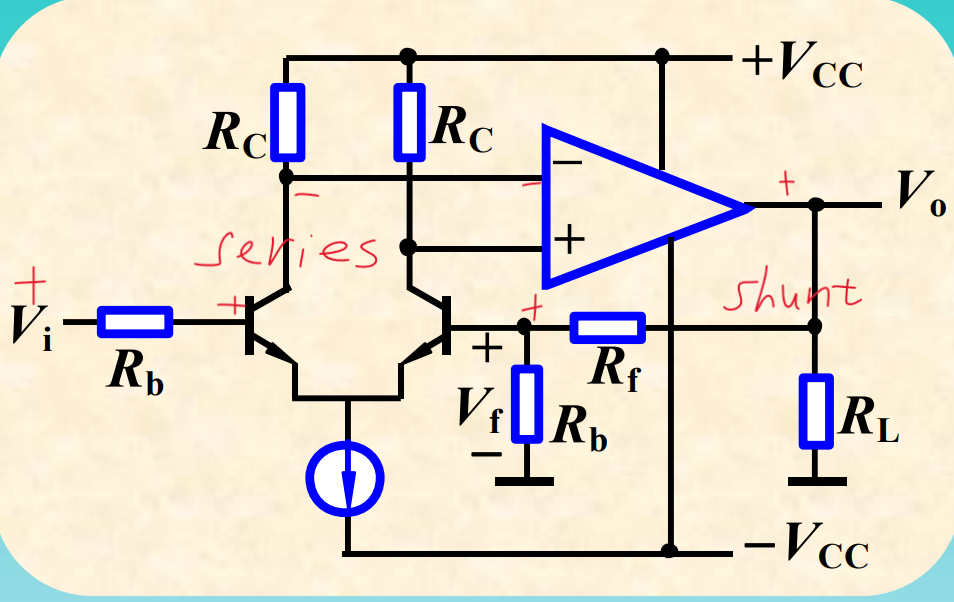
\includegraphics[width=0.6\textwidth]{12.3}
	\caption{Problem 1}
\end{figure}
\noindent Solution:

It's a Series-Shunt-Negative Feedback Circuit. The voltage gain is as follow:
$$
	A_{vf}=\frac{V_o}{V_i}=\frac{V_o}{V_f}=\frac{V_o}{\dfrac{R_b}{R_f+R_b}V_o}=1+\frac{R_f}{R_b}
$$

2.
\begin{figure}[H]
	\centering
	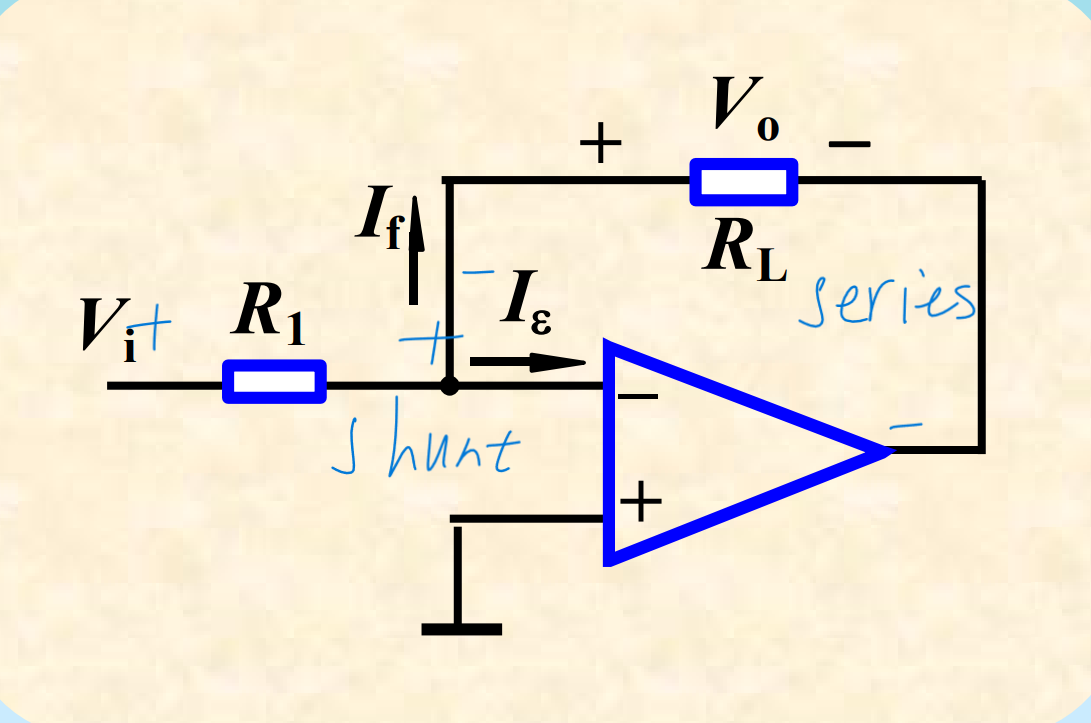
\includegraphics[width=0.6\textwidth]{12.4}
	\caption{Problem 2}
\end{figure}
\noindent Solution:

It's a Shunt-Shunt-Negative Feedback Circuit. The gain is as follow:
$$
	A_{rf}=\frac{V_o}{I_i}=\frac{V_o}{I_f}=R_L\newline
	\Rightarrow A_{vs}=\frac{V_o}{V_i}=\frac{V_o}{I_iR_1}=\frac{R_L}{R_1}
$$

3.
\begin{figure}[H]
	\centering
	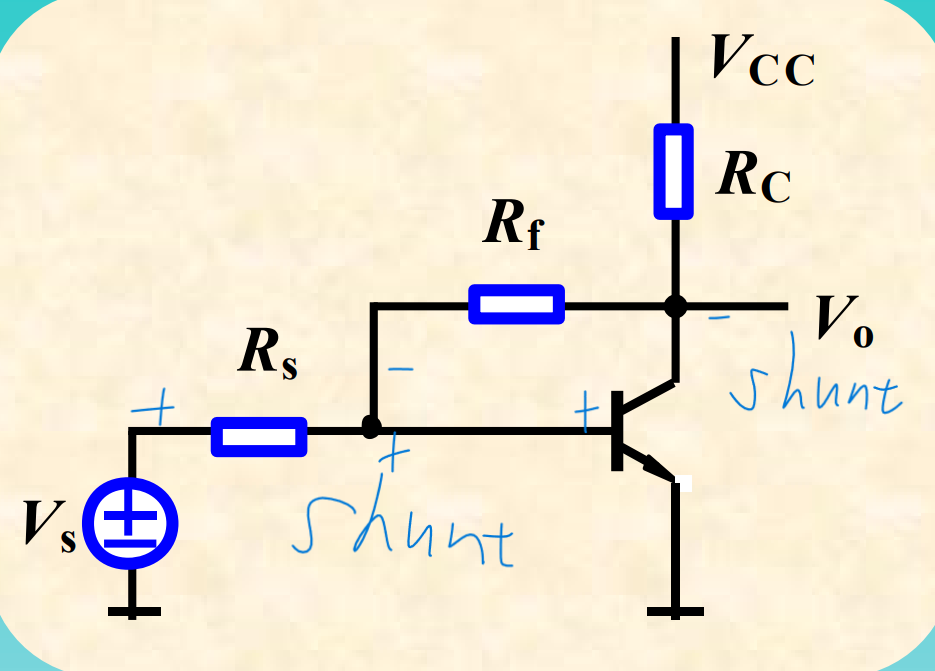
\includegraphics[width=0.6\textwidth]{12.5}
	\caption{Problem 3}
\end{figure}
\noindent Solution:

It's a Shunt-Shunt-Negative Feedback Circuit. The gain is as follow:
$$
	A_{rf}=\frac{V_o}{I_i}=\frac{V_o}{I_f}=-R_f\newline
	\Rightarrow A_{vs}=\frac{V_o}{V_i}=\frac{V_o}{I_iR_s}=-\frac{R_f}{R_s}
$$

4.
\begin{figure}[H]
	\centering
	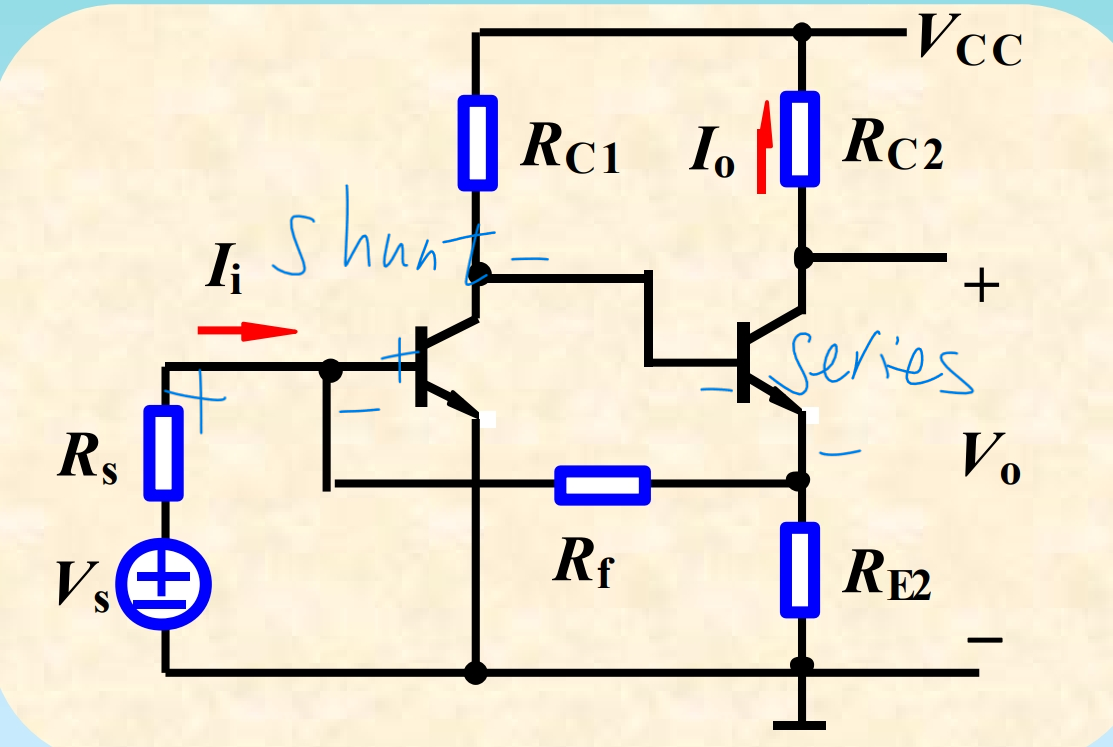
\includegraphics[width=0.6\textwidth]{12.6}
	\caption{Problem 4}
\end{figure}
\noindent Solution:

It's a Shunt-Series-Negative Feedback Circuit. The gain is as follow:
$$
	A_{if}=\frac{I_o}{I_i}=\frac{I_o}{\dfrac{R_{E2}}{R_{E2}+R_f}I_o}=1+\frac{R_f}{R_{E2}}\newline
	\Rightarrow A_{vs}=\frac{V_o}{V_i}=\frac{I_o{R_{C2}}}{I_iR_s}=\frac{R_{C2}}{R_s}(1+\frac{R_f}{R_{E2}})
$$

5. Design feedback network determine its parameter, and connect it with basic amp. Assume that closed-loop is
$$
	A_{vf}=\frac{V_o}{V_i}=-47
$$
\begin{figure}[H]
	\centering
	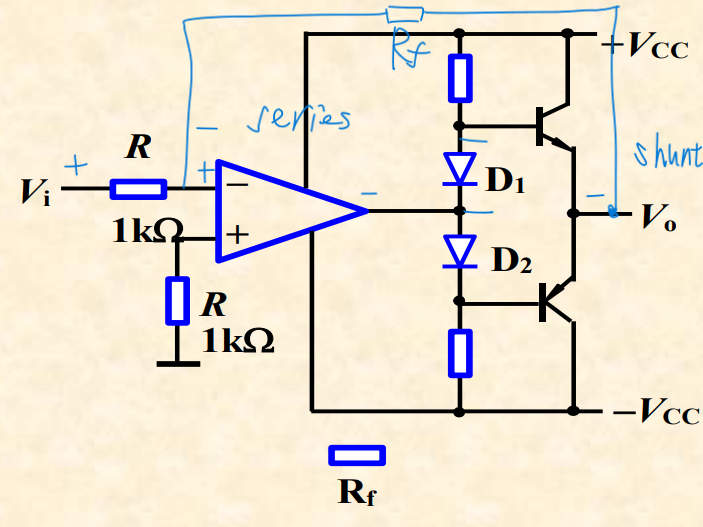
\includegraphics[width=0.6\textwidth]{12.7}
	\caption{Problem 5}
\end{figure}
\noindent Solution:

The designed circuit is in the figure above, It's a Shunt-Shunt-Negative Feedback Circuit. Now we solve the value of resistor $R_f$.
$$
	A_{rf}=\frac{V_o}{I_i}=\frac{V_o}{I_f}=-R_f\Rightarrow A_{vf}=\frac{V_o}{V_i}=\frac{V_o}{I_iR}=-\frac{R_f}{R}\Rightarrow R_f=47\mathrm{k\Omega}
$$
\end{document}